\documentclass{standalone}
% preamble: usepackage, etc.
\begin{document}
\chapter{表格引用}
\section{表格引用}
以下为表格引用格式:

1) table为插入表格提示符;

2) bicaption为表格标题提示符;

3) tabular及后面大括号为表格的列;

4) hline为表格行添加的横线(一般为三线表)。


\begin{table}[htbp]
	\renewcommand{\arraystretch}{0.75}
	\bicaption{数据集}{Datasets Analysis}
	\label{tab_dataset}
	\setlength{\tabcolsep}{1pt}
	\centering 
	\begin{tabular}{lccccccc}
		\hline
		数据集 & \#p. & \#i. & \#c. & \%M. & \#A.\\
		\hline
		A & 48 & 1 & 2 & 67 & \textsl{AU}\\
		Au & 60 & 4 & 2 & 5.5 & \textsl{AU}\\
		B & 625 & 4 & 3 & 4.1 & \textsl{BL}\\  
		W & 49 & 5 & 2 & 94.6 & \textsl{T}\\
		\hline
	\end{tabular}
\end{table}

\section{algorithm算法使用}
以下为algorithm算法的使用方式:

1) caption为算法的标题;

2) label为算法的标签,方便在文章中引用;

3) REQUIRE为算法的输入;

4) ENSURE为算法的输出。


\begin{algorithm}[htbp]
	\caption{语言的艺术中生成模糊规则}
	\begin{algorithmic}[1]
		\REQUIRE \;\\
		$X_{tr} ={a}$,样本集;\\
		$Y_{tr} ={b}$,标签集;\\
		\ENSURE \;\\
		$\bm{B} = (b_{k})$,矩阵;\\
		$\bm{P} = (p_{l})$,概率。 
		\FOR{$j = 1$ to $N_{f}$}
		\FOR{$k = 1$ to $N_{fs}$}
		\STATE 通过式(\ref{eq_fs_parameter})获取$b_{j}$;
		\ENDFOR
		\ENDFOR
	\end{algorithmic}
	\label{alg_iwm_train}
\end{algorithm}



\section{定义引用}

本节为定义定理类的引用,definition为定理提示符,label为定义的标签,方便在文章中引用,enumerate为条件提示符,item表示第几点,如图\ref{fig_13}所示。

引用定义\ref{def_neighbour}的条件得出结论。

\begin{definition}\label{def_neighbour}
	对于$\forall s_{i} \in S$, 满足以下条件:
	\vspace{-3pt}
	\begin{enumerate}
		\item $\bm{a} = (p_{i})$
		\item $\bm{P} = (p_{3})$
	\end{enumerate} 
\end{definition}

\begin{figure}[htbp]
	\centering
	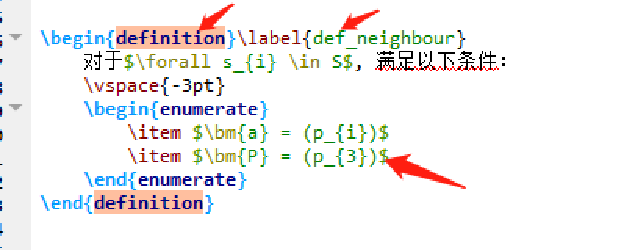
\includegraphics[width = \textwidth]{a15.pdf}
	\bicaption{定理引用教程}{Theorem reference tutorial}
	\label{fig_13}
\end{figure}

\end{document}